% Metamodel: CSP-M
\newcommand{\mcspfragment}{\metaref{CSPFragment}}
\newcommand{\meventsetcspfragment}{\metaref{EventSetCSPFragment}}
\newcommand{\minlinecspfragment}{\metaref{InlineCSPFragment}}
\newcommand{\mprocesscspfragment}{\metaref{ProcessCSPFragment}}
\newcommand{\mcsprefinementproperty}{\metaref{CSPRefinementProperty}}
\newcommand{\mcspprocesssource}{\metaref{CSPProcessSource}}
\newcommand{\mcspcontextsource}{\metaref{CSPContextSource}}


\section{Introduction}\label{ssec:core-metamodel-intro}
\subsection{How to read the rest of this chapter}\label{ssec:core-metamodel-intro-readme}

Each section, except this one,
introduces a group of top-level \langname{}
functionality in a top-down manner.  These sections contain:

\begin{itemize}
\item
	a class diagram representing the Ecore classes, enumerations, and other
	components that make up the group being discussed;
\item
	descriptions of the components being shown in the class diagram;
\item
	where relevant, examples of the components in terms of the concrete
	syntaxes of \langname.
\end{itemize}

\section{Top-level}\label{ssec:core-metamodel-top}
% !TEX root=../../robocert.tex
\begin{figure}[htb]
  \centering
  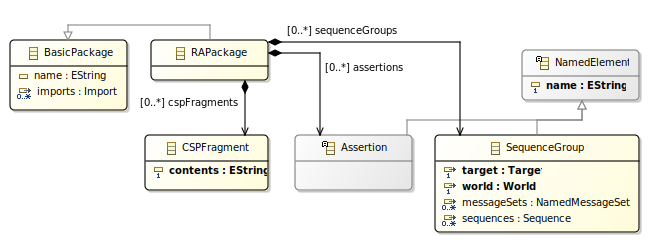
\includegraphics[width=.85\textwidth]{diagrams/Top}
  \caption{Class diagram for the top of the \langname{} metamodel.}
  \label{fig:metamodel-top}
\end{figure}

\Cref{fig:metamodel-top} is the top-level metamodel diagram for \langname.

Each \langname{} script contains an \mrapackage,\footnote{\mrapackage{} stands
  for `RoboStar Assertions package'; we use this name because \mrcpackage{} is
  already used for RoboChart packages.}
which is a type of RoboStar \mbasicpackage.
Each \mrapackage{} can contain zero or more of each of these types of content:

\begin{itemize}
\item
  \msequencegroup:
  a sequence diagram group
  (see \cref{sec:metamodel-sequences});
\item
  \mcspgroup:
  a CSP fragment, currently not bound to a particular process
  \todo{this will change};
\item
  \massertion:
  an assertion
  (see \cref{sec:core-metamodel-assertions}).
\end{itemize}

%%% Local Variables:
%%% mode: latex
%%% TeX-master: "../../robocert"
%%% End:


%%% Local Variables:
%%% mode: latex
%%% TeX-master: "../robocert"
%%% End:
